% Options for packages loaded elsewhere
\PassOptionsToPackage{unicode}{hyperref}
\PassOptionsToPackage{hyphens}{url}
\PassOptionsToPackage{dvipsnames,svgnames,x11names}{xcolor}
%
\documentclass[
  number,
  preprint,
  3p]{elsarticle}

\usepackage{amsmath,amssymb}
\usepackage{iftex}
\ifPDFTeX
  \usepackage[T1]{fontenc}
  \usepackage[utf8]{inputenc}
  \usepackage{textcomp} % provide euro and other symbols
\else % if luatex or xetex
  \usepackage{unicode-math}
  \defaultfontfeatures{Scale=MatchLowercase}
  \defaultfontfeatures[\rmfamily]{Ligatures=TeX,Scale=1}
\fi
\usepackage{lmodern}
\ifPDFTeX\else  
    % xetex/luatex font selection
\fi
% Use upquote if available, for straight quotes in verbatim environments
\IfFileExists{upquote.sty}{\usepackage{upquote}}{}
\IfFileExists{microtype.sty}{% use microtype if available
  \usepackage[]{microtype}
  \UseMicrotypeSet[protrusion]{basicmath} % disable protrusion for tt fonts
}{}
\makeatletter
\@ifundefined{KOMAClassName}{% if non-KOMA class
  \IfFileExists{parskip.sty}{%
    \usepackage{parskip}
  }{% else
    \setlength{\parindent}{0pt}
    \setlength{\parskip}{6pt plus 2pt minus 1pt}}
}{% if KOMA class
  \KOMAoptions{parskip=half}}
\makeatother
\usepackage{xcolor}
\setlength{\emergencystretch}{3em} % prevent overfull lines
\setcounter{secnumdepth}{5}
% Make \paragraph and \subparagraph free-standing
\ifx\paragraph\undefined\else
  \let\oldparagraph\paragraph
  \renewcommand{\paragraph}[1]{\oldparagraph{#1}\mbox{}}
\fi
\ifx\subparagraph\undefined\else
  \let\oldsubparagraph\subparagraph
  \renewcommand{\subparagraph}[1]{\oldsubparagraph{#1}\mbox{}}
\fi


\providecommand{\tightlist}{%
  \setlength{\itemsep}{0pt}\setlength{\parskip}{0pt}}\usepackage{longtable,booktabs,array}
\usepackage{calc} % for calculating minipage widths
% Correct order of tables after \paragraph or \subparagraph
\usepackage{etoolbox}
\makeatletter
\patchcmd\longtable{\par}{\if@noskipsec\mbox{}\fi\par}{}{}
\makeatother
% Allow footnotes in longtable head/foot
\IfFileExists{footnotehyper.sty}{\usepackage{footnotehyper}}{\usepackage{footnote}}
\makesavenoteenv{longtable}
\usepackage{graphicx}
\makeatletter
\def\maxwidth{\ifdim\Gin@nat@width>\linewidth\linewidth\else\Gin@nat@width\fi}
\def\maxheight{\ifdim\Gin@nat@height>\textheight\textheight\else\Gin@nat@height\fi}
\makeatother
% Scale images if necessary, so that they will not overflow the page
% margins by default, and it is still possible to overwrite the defaults
% using explicit options in \includegraphics[width, height, ...]{}
\setkeys{Gin}{width=\maxwidth,height=\maxheight,keepaspectratio}
% Set default figure placement to htbp
\makeatletter
\def\fps@figure{htbp}
\makeatother

\usepackage{lineno}\linenumbers
\makeatletter
\makeatother
\makeatletter
\makeatother
\makeatletter
\@ifpackageloaded{caption}{}{\usepackage{caption}}
\AtBeginDocument{%
\ifdefined\contentsname
  \renewcommand*\contentsname{Table of contents}
\else
  \newcommand\contentsname{Table of contents}
\fi
\ifdefined\listfigurename
  \renewcommand*\listfigurename{List of Figures}
\else
  \newcommand\listfigurename{List of Figures}
\fi
\ifdefined\listtablename
  \renewcommand*\listtablename{List of Tables}
\else
  \newcommand\listtablename{List of Tables}
\fi
\ifdefined\figurename
  \renewcommand*\figurename{Figure}
\else
  \newcommand\figurename{Figure}
\fi
\ifdefined\tablename
  \renewcommand*\tablename{Table}
\else
  \newcommand\tablename{Table}
\fi
}
\@ifpackageloaded{float}{}{\usepackage{float}}
\floatstyle{ruled}
\@ifundefined{c@chapter}{\newfloat{codelisting}{h}{lop}}{\newfloat{codelisting}{h}{lop}[chapter]}
\floatname{codelisting}{Listing}
\newcommand*\listoflistings{\listof{codelisting}{List of Listings}}
\makeatother
\makeatletter
\@ifpackageloaded{caption}{}{\usepackage{caption}}
\@ifpackageloaded{subcaption}{}{\usepackage{subcaption}}
\makeatother
\makeatletter
\@ifpackageloaded{tcolorbox}{}{\usepackage[skins,breakable]{tcolorbox}}
\makeatother
\makeatletter
\@ifundefined{shadecolor}{\definecolor{shadecolor}{rgb}{.97, .97, .97}}
\makeatother
\makeatletter
\makeatother
\makeatletter
\makeatother
\journal{Journal Name}
\ifLuaTeX
  \usepackage{selnolig}  % disable illegal ligatures
\fi
\usepackage[]{natbib}
\bibliographystyle{elsarticle-num}
\IfFileExists{bookmark.sty}{\usepackage{bookmark}}{\usepackage{hyperref}}
\IfFileExists{xurl.sty}{\usepackage{xurl}}{} % add URL line breaks if available
\urlstyle{same} % disable monospaced font for URLs
\hypersetup{
  pdftitle={Assessment of drought impact over land cover in continental Chile by the analysis of water supply and demand from the ERA5-Land and MODIS},
  pdfauthor={Francisco Zambrano},
  pdfkeywords={drought, land cover change, satellite},
  colorlinks=true,
  linkcolor={blue},
  filecolor={Maroon},
  citecolor={Blue},
  urlcolor={Blue},
  pdfcreator={LaTeX via pandoc}}

\setlength{\parindent}{6pt}
\begin{document}

\begin{frontmatter}
\title{Assessment of drought impact over land cover in continental Chile
by the analysis of water supply and demand from the ERA5-Land and MODIS}
\author[1]{Francisco Zambrano%
\corref{cor1}%
\fnref{fn1}}
 \ead{francisco.zambrano@umayor.cl} 

\affiliation[1]{organization={Universidad Mayor, Hémera Centro de
Observación de la Tierra, Facultad de Ciencias, Escuela de Ingeniería en
Medio Ambiente y Sustentabilidad},city={Santiago,
Chile},postcode={7500994},postcodesep={}}

\cortext[cor1]{Corresponding author}
\fntext[fn1]{This is the first author footnote.}
        
\begin{abstract}
Human-induced greenhouse gas emissions have increased the frequency
and/or intensity of weather and climate extremes. Central Chile has been
affected by a persistent drought which is impacting the hydrological
system and vegetation development. The region has been the focus of
research studies due to the diminishing water supply, this persistent
period of water scarcity has been defined as a ``mega drought''.
Nevertheless, our results evidence that the water deficit has expanded
beyond. Our goal is to analyze the impact of drought, measured by
drought indices of water supply/demand and vegetation status, in the
LULCC (land use land cover change) over continental Chile. For the
analysis, continental Chile was divided into five zones according to a
latitudinal gradient: ``Norte Grande'', ``Norte Chico'', ``Zona
Central'', ``Zona Sur'', and ``Zona Austral''. We used monthly climatic
re-analysis variables for precipitation, temperature and soil moisture
for 1981-2023 from ERA5-Land; and MODIS (Moderate-Resolution Imaging
Spectroradiometer) product MCD12Q1 for land cover for 2001-2021, and the
NDVI vegetation index from product MOD13A2 collection 6.1 for 2000-2023,
both from collection 6.1. We estimated atmospheric evaporative demand
(AED) by combining the Hargreaves-Samani equation with the ERA5-Land
temperature. We derived the drought indices SPI (Standardized
Precipitation Index), SPEI (Standardized Precipitation
Evapotranspiration Index), EDDI (Evaporative Demand Drought Index), zcSM
(standardized anomaly of cumulative soil moisture), and the zcNDVI
(standardized anomaly of cumulative NDVI). These indices were calculated
for time scales of 1, 3, 6, 12, 24, and 36 months, except for zcNDVI (1,
3, and 6 months). We analyzed the temporal correlation of SPI, SPEI,
EDDI, and zcSM with zcNDVI to have insights into the impact of water
supply and demand on vegetation. Our results showed that LULCC had an
increasing trend of 412 {[}km2yr−1{]} of forest expansion in the ``Zona
Sur'', together with a decreasing trend of 24 {[}km2yr−1{]} of cropland
contraction in the ``Zona Central'' meanwhile the ``Zona Sur'' showed an
increase of 31 {[}km2yr−1{]}, and a contraction of 80 {[}km2yr−1{]} of
bare soil in the ``Zona Austral''. The EDDI was the less correlated
index for the five macro zones and the five types of land cover, showing
that the temperature in Chile has little impact on vegetation. Higher
r-squared values, between 0.5 and 0.8, were obtained at ``Norte Chico''
and ``Zona Central'' for the land cover types of savanna, shrubland,
grassland, and croplands for the indices SPEI and zcSM at time scales of
12 and 24 months. The forest type reaches a r-squared of
\textasciitilde0.5 for zcSM of 12 months. The results indicate that the
``Norte Chico'' and ``Zona Central'' are the most sensitive regions to
water supply deficits longer than a year, potentially explained by a low
capacity of water storage in those zones that should be further
investigated.
\end{abstract}





\begin{keyword}
    drought \sep land cover change \sep 
    satellite
\end{keyword}
\end{frontmatter}
    \ifdefined\Shaded\renewenvironment{Shaded}{\begin{tcolorbox}[frame hidden, boxrule=0pt, breakable, interior hidden, borderline west={3pt}{0pt}{shadecolor}, enhanced, sharp corners]}{\end{tcolorbox}}\fi

\hypertarget{introduction}{%
\section{Introduction}\label{introduction}}

The sixth assessment report (AR6) of the IPCC \citep{IPCC2023} indicates
that human-induced greenhouse gas emissions have increased the frequency
and/or intensity of some weather and climate extremes, and the evidence
has been strengthened since AR5 \citep{IPCC2013}. There is high
confidence that increasing global warming can expand the land area
affected by increasing drought frequency and severity
\citep{IPCCCH112021}. Furthermore, drought increases tree mortality and
triggers changes in land cover and, consequently, land use, thus
impacting ecosystems \citep{Crausbay2017}. Nevertheless, there is a lack
of understanding of how the alteration in water supply and demand is
affecting land cover transformations.

Precipitation is the primary driver of drought and is intensified by
temperature \citep{Luo2017}. Drought impacts soil moisture, hydrological
regimes, and vegetation productivity. Initially, drought was commonly
classified as meteorological, hydrological, and agricultural
\citep{Wilhite1985}. Lately, \citep{Loon2016} and
\citep{AghaKouchak2021} have given an updated definition of drought for
the Anthropocene, suggesting that it should be considered the feedback
of humans' decisions and activities that drives the anthropogenic
drought. Even though it has been argued that those definitions do not
fully address the ecological dimensions of drought. \citep{Crausbay2017}
proposed the ecological drought definition as \emph{``an episodic
deficit in water availability that drives ecosystems beyond thresholds
of vulnerability, impacts ecosystem services, and triggers feedback in
natural and/or human systems''}. Moreover, many ecological studies have
misinterpreted how to characterize drought, for example, sometimes
considering ``dry'' conditions as ``drought'' \citep{Slette2019}. On the
other hand, the AR6 \citep{IPCC2023} states that even if global warming
is stabilized at 1.5°--2°C, many parts of the world will be impacted by
more severe agricultural and ecological droughts. Then, there is a
challenge in conducting drought research, especially to evaluate its
impact on ecosystems.

Chile has been facing a persistent rainfall deficit for more than a
decade \citep{Garreaud2017}, which has impacted vegetation development
\citep{Zambrano2023} and the hydrological system \citep{Boisier2018}.
Current drought conditions have affected crop productivity
\citep{Zambrano2016, Zambrano2018}, forest development
\citep{Miranda2020, Venegas2018}, forest fire occurrence
\citep{UrrutiaJalabert2018}, land cover change \citep{Fuentes2021},
water supply in watersheds \citep{AlvarezGarreton2021}, and have had
economic impacts \citep{Fernandez2023}. In 2019--2020, the drought
severity reached an extreme condition in Central Chile (30--34°S) not
seen for at least 40 years, and the evidence indicates that the impact
is transversal to the land cover classes of forest, grassland, and
cropland \citep{Zambrano2023}. The prolonged lack of precipitation in
Central Chile is producing changes in ecosystem dynamics that must be
studied.

For the spatiotemporal assessment of drought impact (i.e., by water
supply and demand) on land cover changes, we need climatic realiable
variables such as precipitation, temperature, soil moisture, land cover,
and vegetation status. For developing countries like Chile, the weather
networks present several disadvantages, such as gaps, a short history,
and low-quality data. Reanalysis data, as the ERA5-Land (ERA5L)
\citep{MunozSabater2021} provides hourly climatic information
(precipitation, temperature, and soil moisture) without gaps since 1950
with global extension. ERA5L has already been used for drought
assessment using the Standardized Precipitation-Evapotranspiration Index
(SPEI) \citep{Nouri2023} and for flash drought \citep{Wang2023} by
analyzing soil mositure and evapotranspiration. On the other hand,
satellite remote sensing \citep{West2019, AghaKouchak2015} is the
primary method to evaluate how drought impacts vegetation dynamics.
Vegetation drought indices (VDI) are commonly used as proxies of
productivity \citep{Paruelo2016, Schucknecht2017}, which can be derived
from the MODIS (Moderate-Resolution Imaging Spectroradiometer). Besides,
land use and land cover (LULC) change can be driven by drought
\citep{Tran2019, Akinyemi2021}. To analyze these changes, multiple LULC
products exist \citep{Grekousis2015}, one of those that provides time
series since 2001 is the MCD12Q1 \citep{Friedl2019} from MODIS. The
variation in water supply and demand is finally reflected in the total
water storage (TWS). The TWS can be retrieved by the Gravity Recovery
and Climate Experiment (GRACE), which allows analyzing water
availability changes at coarse resolution \citep{Ahmed2014, Ma2017}. We
can use climatic reanalysis (ERA5L) and vegetation data (MODIS) to
derive drought indices of supply (i.e., precipitation) and demand (i.e.,
temperature) and thus evaluate the impact of drought on LULC changes.
Further, the TWS can be assessed with regard to the changes in water
supply and demand to gain insight into the impact on water storage.

To evaluate meteorological drought (i.e., water supply), the World
Meteorological Organization (WMO; \citep{WMO2012}) recommends the
Standardized Precipitation Index (SPI; \citep{Mckee1993}), a multiscalar
drought index that allows to monitor precipitation deficits from short-
to long-term. Following the same approach, \citep{Vicente-Serrano2010}
incorporates into the SPI the effect of temperature through the use of
potential evapotranspiration, thus proposing the SPEI (Standardized
Precipitation Evapotranspiration Index). Similarly, to evaluate solely
the evaporative demand driven by temperature, \citep{Hobbins2016} and
\citep{McEvoy2016} came up with the Evaporative Demand Drought Index
(EDDI). For vegetation, in a similar manner as the SPI, SPEI and EDDI;
~\citep{Zambrano2018} proposed the zcNDVI, a standardized anomaly of the
cumulative Normalized Difference Vegetation Index (NDVI), which could be
acumulated over the growing season or any period (e.g., months),
resulting in a multiscalar drought index. For soil moisture, several
drought indices exist, such as the Soil Moisture Deficit Index (SDMI) a
normalized index \citep{Narasimhan2005} and the Soil Moisture
Agricultural Drought Index (SMADI) \citep{Souza2021} which is a
normalized index using vegetation, land surface temperature, and a
vegetation condition index (VCI, \citep{Kogan1995}). From TWS, we can
estimate the standardized terrestrial water storage index (STI)
\citep{Cui2021}, a standardized anomaly that follows the methodology of
the SPI, SPEI, EDDI, and zcNDVI. Thereby, we have drought indices for
water supply, demand, and storage, which can help to make a
comprehensive assessment of drought.

In this research, we aim to analyze the impact of drought on different
types of land cover classes in continental Chile by combining
environmental variables such as biomass productivity, and water demand
and supply gathered from earth observation products. The specific
objectives of the study are: i) to calculate multi-scalar drought
indices for water demand and supply for 1981--2023; ii) to evaluate LULC
change for 2001--2021 and its relation to drought indices; iii) to
analyze the relationship of a proxy of biomass (zcNDVI) with drought
indices; and iv) to assess if the observed changes in the drought
indices are linked to the TWS.

\hypertarget{study-area}{%
\section{Study area}\label{study-area}}

\begin{figure}[ht]

{\centering 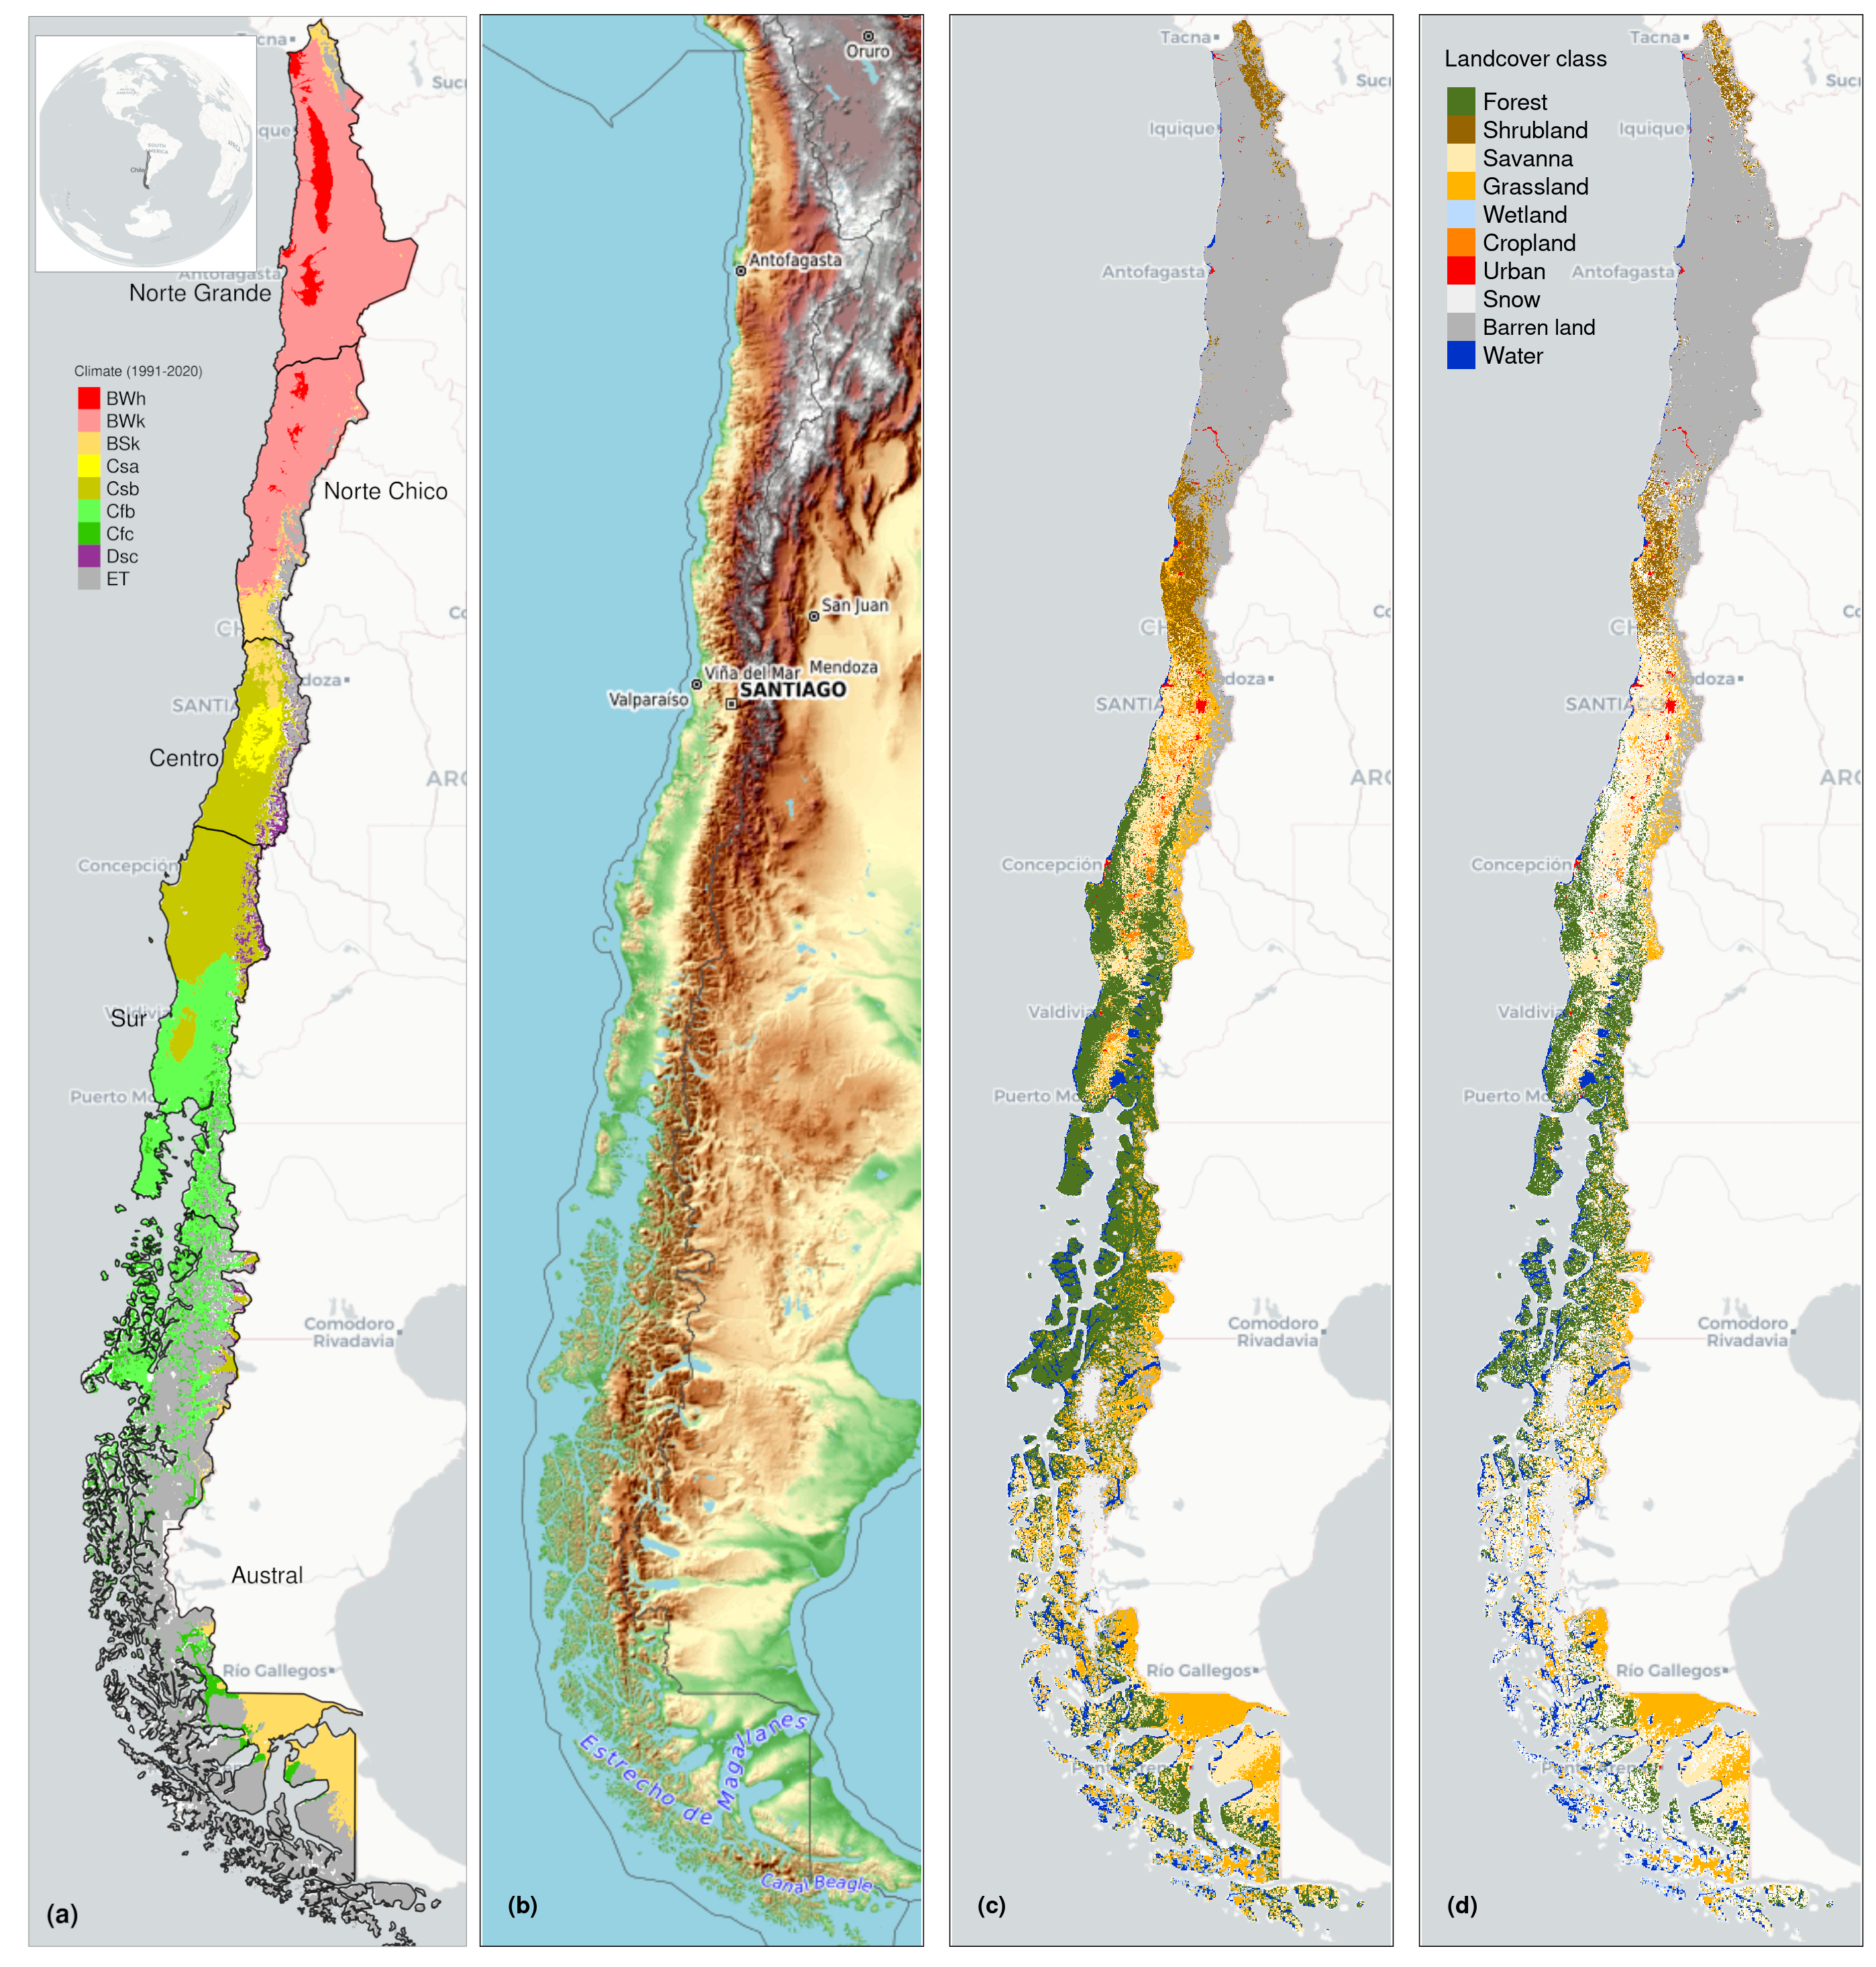
\includegraphics[width=0.8\textwidth,height=\textheight]{../output/figs/map_study_con_landcover.png}

}

\caption{(a) Chile and the five zones ``norte grande'', ``norte chico'',
``zona central'', ``zona sur'', and ``zona austral''. (b) Topography
reference map. (c) Land cover classes for 2021. (d) Persistent land
cover classes (\textgreater{} 80\%) for 2001-2021.}

\end{figure}

\hypertarget{materials-and-methods}{%
\section{Materials and Methods}\label{materials-and-methods}}

\hypertarget{data}{%
\subsection{Data}\label{data}}

\hypertarget{earth-observation-data}{%
\subsubsection{Earth observation data}\label{earth-observation-data}}

\hypertarget{in-situ-data}{%
\subsubsection{in-situ data}\label{in-situ-data}}

\hypertarget{drought-indices-for-water-demand-and-supply}{%
\subsection{Drought indices for water demand and
supply}\label{drought-indices-for-water-demand-and-supply}}

\hypertarget{analysis-of-a-biomass-proxy-with-drought-indices-of-supply-and-demand}{%
\subsection{Analysis of a biomass proxy with drought indices of supply
and
demand}\label{analysis-of-a-biomass-proxy-with-drought-indices-of-supply-and-demand}}

\hypertarget{lulc-change-for-2001-2021-and-its-relation-with-water-supply-and-demand}{%
\subsection{LULC change for 2001-2021 and its relation with water supply
and
demand}\label{lulc-change-for-2001-2021-and-its-relation-with-water-supply-and-demand}}

!{[}Proportion of land cover class from the persistent land cover for
2001-2021 (\textgreater80\%) per macrozone.

\begin{figure}

\begin{minipage}[t]{0.47\linewidth}

{\centering 

\raisebox{-\height}{

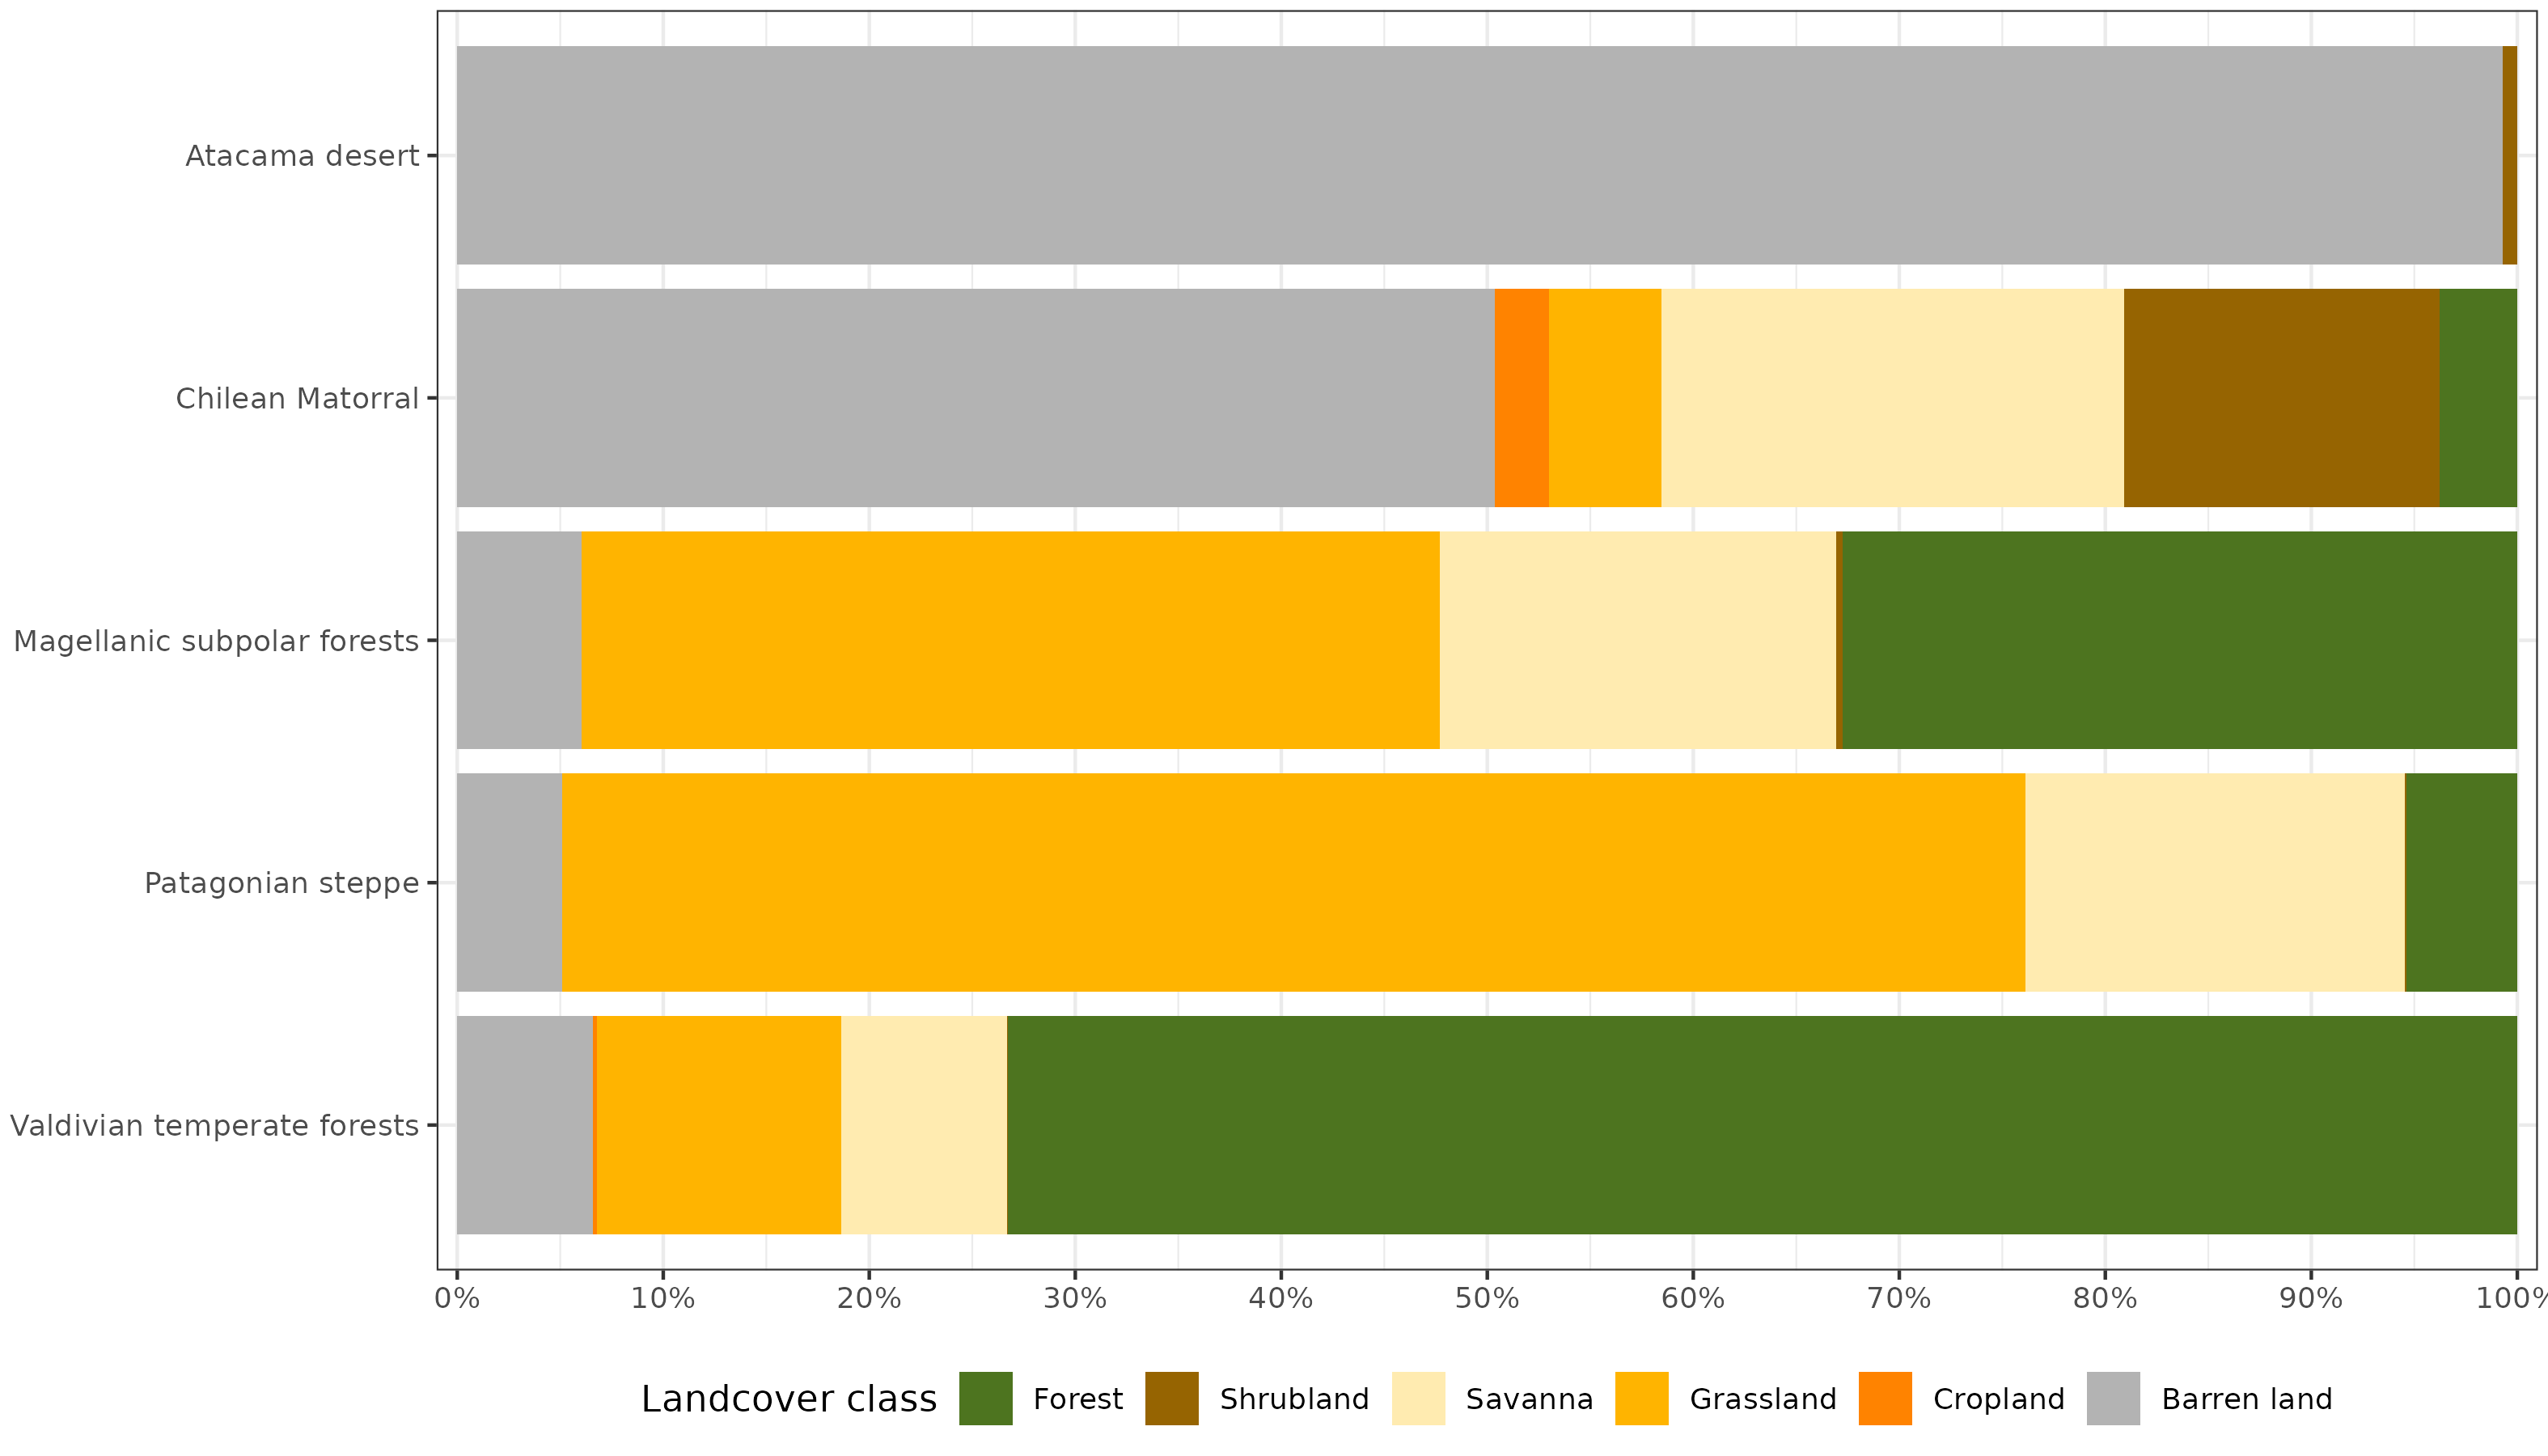
\includegraphics[width=7cm,height=\textheight]{../output/figs/LC_pers80_per_macrozone.png}

}

}

\end{minipage}%
%
\begin{minipage}[t]{0.53\linewidth}

{\centering 

\raisebox{-\height}{

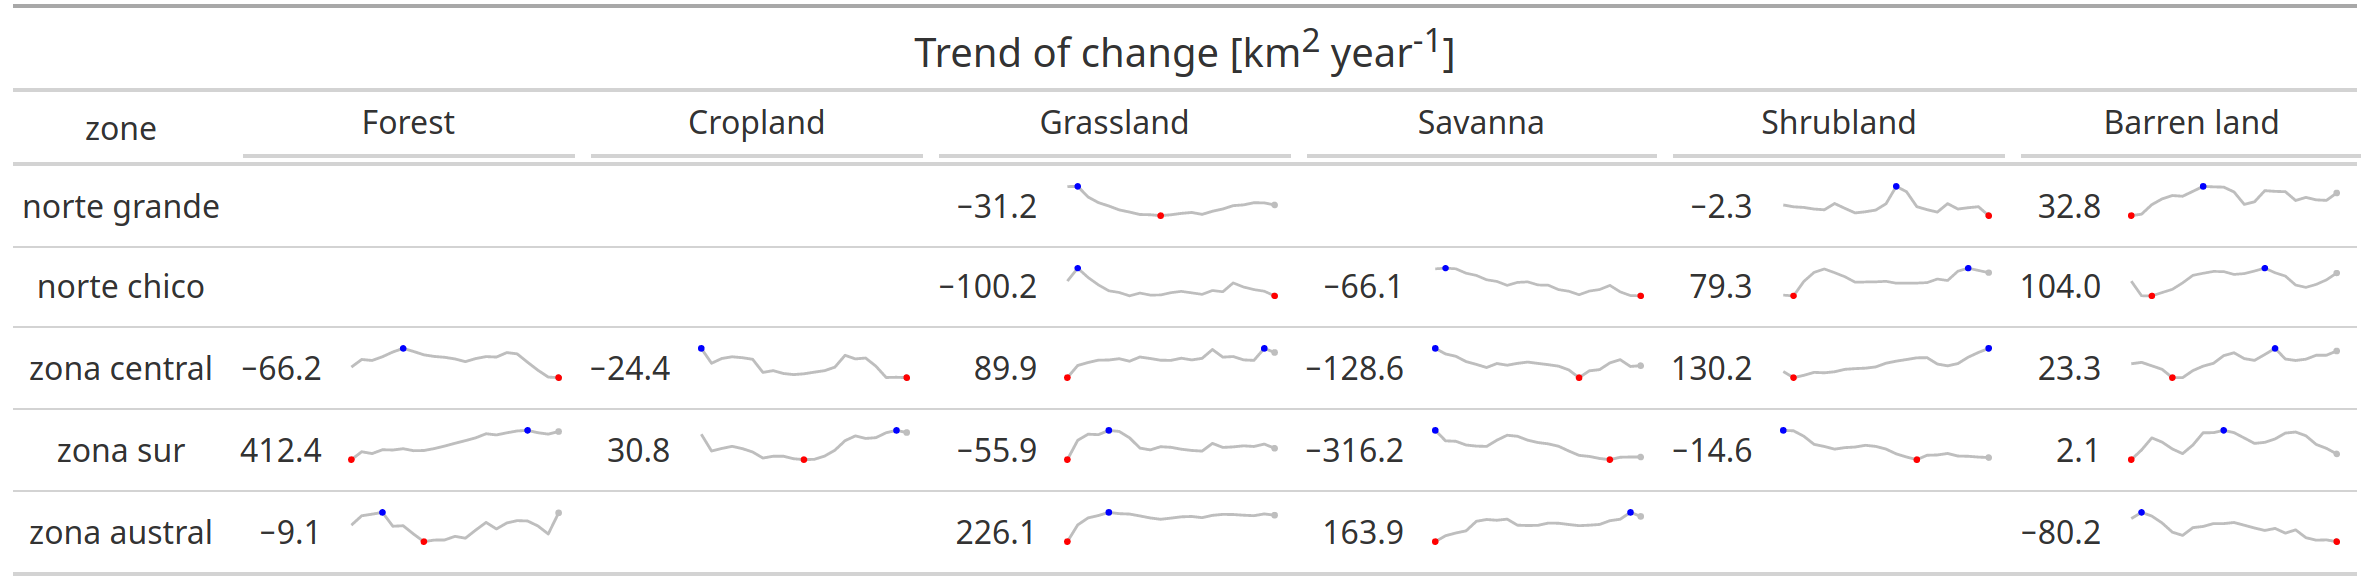
\includegraphics[width=8cm,height=\textheight]{../output/figs/table_var_landcover_macro.png}

}

}

\end{minipage}%

\caption{\label{fig-elephants}Proportion of land cover class from the
persistent land cover for 2001-2021 (\textgreater80\%) per macrozone.
The table on the left shows the linear change trend next to time-series
plot of surface, per land cover class (IGBP MCD12Q1.006) for 2001-2021
through the fives zones on continental Chile. Blue dots on the plots
indicate the maximum and red dots minimum surface reach.}

\end{figure}

\hypertarget{total-water-storage-and-drought-indices}{%
\subsection{Total water storage and drought
indices}\label{total-water-storage-and-drought-indices}}

Terrestrial Water Storage (TWS) is defined as the total amount of water
stored on land that includes any natural or artificial water bodies,
such as groundwater, soil moisture, rivers, lakes, snowpack, ice, and
biomass water \citep{Humphrey2023, Deng2023}. TWS changes evidence the
effects of multiple water fluxes on the hydrological cycle
\citep{Deng2023}. These are reflected in the temporal variation of
observations of the Earth's gravitational field
\citep{Abolafia2021, Sabzehee2023} and, in recent decades, the twin
Gravity Recovery and Climate Experiment (GRACE) satellites and their
Follow-On mission (GRACE-FO) have provided valuable results on globally
distributed TWS anomalies \citep{Tapley2019, Ferreira2023}. The GRACE
mission was launched in March 2002 and was operational until October
2017 \citep{Ramjeawon2022}. Then its GRACE Follow-On successor was
launched in May 2018 \citep{Landerer2020, Yin2022}. The information
provided by these satellites is used to construct monthly maps of the
Earth's average gravity field, providing details of the movement of
water masses or water mass anomaly estimates relative to the long-term
average gravity field \citep{Humphrey2023, Wahr2004}.

In this study, RL06.1\_V3 GRACE mascon (mass concentration) monthly
solutions were used, which are provided by the Jet Propulsion Laboratory
(JPL-M, https://grace.jpl.nasa.gov). Each GRACE Tellus monthly grid at
0.5 degrees represents the deviation of surface mass for that month
relative to a reference time average (2004-2009 baseline), which is
subtracted from all other monthly grids to provide terrestrial water
storage anomalies (TWSA) \citep{Ramjeawon2022, Yin2022}. This JPL-M
version of the data employs a Coastal Resolution Improvement (CRI)
filter that reduces signal leakage errors across coastlines
\citep{Wiese2019, Wiese2016}. Although the mascon solutions greatly
reduced leakage errors, a gain factor, which is used to enhance the
spatial resolution, was applied to the dataset as recommended for
hydrological studies \citep{Ramjeawon2022, Yin2022}. The water storage
and height anomalies are given in Equivalent Water Height or Thickness
units (EWH, cm) \citep{Sabzehee2023}, and their temporal resolution
monthly is from April 2002 to May 2023.

\hypertarget{validation-of-era5-land-variables}{%
\subsection{Validation of ERA5-Land
variables}\label{validation-of-era5-land-variables}}

\hypertarget{results}{%
\section{Results}\label{results}}

\hypertarget{drought-indices-for-water-demand-and-supply-1}{%
\subsection{Drought indices for water demand and
supply}\label{drought-indices-for-water-demand-and-supply-1}}

\hypertarget{biomass-proxy-with-drought-indices-of-supply-and-demand}{%
\subsection{Biomass proxy with drought indices of supply and
demand}\label{biomass-proxy-with-drought-indices-of-supply-and-demand}}

\hypertarget{lulc-change-for-2001-2021-and-its-relation-with-water-supply-and-demand-1}{%
\subsection{LULC change for 2001-2021 and its relation with water supply
and
demand}\label{lulc-change-for-2001-2021-and-its-relation-with-water-supply-and-demand-1}}

\hypertarget{total-water-storage-tws-and-drought-indices}{%
\subsection{Total water storage (TWS) and drought
indices}\label{total-water-storage-tws-and-drought-indices}}

\hypertarget{validation-of-era5-land-variables-1}{%
\subsection{Validation of ERA5-Land
variables}\label{validation-of-era5-land-variables-1}}

\hypertarget{discussion}{%
\section{Discussion}\label{discussion}}

\hypertarget{conclusion}{%
\section{Conclusion}\label{conclusion}}


\renewcommand\refname{References}
  \bibliography{references.bib}


\end{document}
